\documentclass[conference, compsoc]{IEEEtran}

\usepackage{graphicx}
\usepackage{makeidx}
\usepackage{url}
\usepackage{subcaption}
\usepackage{enumerate}
\usepackage{enumitem}
\usepackage{ifthen}
\usepackage{amssymb}
\usepackage{dsfont}
\usepackage{multicol}
\usepackage[hidelinks]{hyperref}
\usepackage{amsmath}
\usepackage{multirow}
\usepackage{booktabs}
\usepackage{csvsimple}

% One command per author:
\newboolean{showcomments}
\setboolean{showcomments}{true}
%\setboolean{showcomments}{false}
\ifthenelse{\boolean{showcomments}}
 { \newcommand{\mynote}[2]{
      \fbox{\bfseries\sffamily\scriptsize#1}
        {\small$\blacktriangleright$\textsf{\emph{#2}}$\blacktriangleleft$}}}
        { \newcommand{\mynote}[2]{}}


\newcommand{\xb}[1]{\mynote{Xavier}{#1}}
\newcommand{\ced}[1]{\mynote{Cedric}{#1}}

\newcommand{\figref}[1]{Figure~\ref{fig:#1}}
\newcommand{\tabref}[1]{Table~\ref{tab:#1}}
\newcommand{\secref}[1]{Section~\ref{sec:#1}}
\newcommand{\alref}[1]{Algorithm~\ref{alg:#1}}
\newcommand{\lstref}[1]{Listing~\ref{lst:#1}}

\title{Impact of Artifact Renaming on Software Change Metrics}

\author{
\IEEEauthorblockN{Jean-R\'emy Falleri, Pierre Chanson, Matthieu Foucault and Xavier Blanc}
\IEEEauthorblockA{
University of Bordeaux \\
LaBRI, UMR 5800\\
F-33400, Talence, France\\
Email: \{falleri,mfoucaul,xblanc\}@labri.fr, pierre.chanson@etu.u-bordeaux.fr}
}

\begin{document}

\maketitle
\begin{abstract}
Change metrics, such as Churn or Number of Developers, are good indicators for Software quality, as it has been observed by several studies. However, as these metrics are computed from the changes performed to a software artifact, their value may be skewed in case of artifact renaming, which can therefore be a important threat to validity. 
This issue is underestimated in most of the existing software study. We therefore propose to assess its impact in this paper. To that extent, we have performed an empirical study on five open-source programs with the intent to evaluate the amount of renaming and their effect on change metrics. We observed that the renaming can significantly alter the metrics for some projects. We also noticed that this effect can be minimizing by following some simple guidelines we present in this paper. 
\end{abstract}


\section{Introduction}
\label{sec:intro}

L'accès aux dépôts logiciels a rendu possible de nombreux travaux de recherche sur l'évolution logicielle. Plus particulièrement, les dépôts de code source gérés par des outils de contrôle de versions (Version Control System, VCS, comme SVN, Mercurial ou encore Git) contiennent l'historique de construction d'un logiciel. Principalement dans le domaine du ``Reverse Engineering'', la compréhension des choix des développeurs lors de la création d'un logiciel, des études se basent sur l'analyse de ces historiques. Ces études entrent dans le cadre des études ``MSR'' (Minning Software Repository). De même, la prédiction de bugs, un des défis connus du Génie Logiciel dont le but est de prédire le nombre de bugs et leur localisation dans la prochaine version d'un logiciel, utilise des informations contenu dans l'historique d'un projet. Cette étude se base sur les métriques de procédés comme prédicateurs de bugs. Les métriques de procédés se concentrent sur l'évolution d'un logiciel et mesurent les modifications subies par les entités d'un code source durant leur cycle de vie. L'hypothèse principale étant que la manière dont les entités du code ont changé a un impact majeur sur la qualité de leur prédiction de bugs.\\
Or au cours de son histoire, un fichier peut être renommé et/ou déplacé dans un autre dossier du projet.\\
Théoriquement, si le renommage d'un fichier à un moment donné de son histoire n'est pas pris en compte, le calcul d'une métrique de procédé sur ce fichier sera faussé. En effet, si on identifie le fichier par son nom, on perdra les informations récoltées avant le renommage. Par ailleurs on peut penser que le refactoring, dont le renommage de fichiers, est très présent dans le développement des logiciels à succès d'aujourd'hui. En pratique, nous n'avons pas de chiffres pour le montrer.\\ 
Dans un premier temps nous effectuerons une étude de l'existant sur les méthodes utilisées pour détecter le refactoring, les logiciels qui ont été étudié, les métriques de procédés ainsi que les VCS. Puis nous choisirons un ensemble de projets cohérent pour faire nos propres expérimentations, nous définirons un niveau de granularité et nous ferons une analyse manuelle des projets choisis pour récupérer les renommages réels. Par la suite, nous définirons un modèle et nous utiliserons un outil pour récupérer les renommages. Enfin, nous définirons comment calculer certaines métriques de procédés et mesurerons l'impact du renommage. Les résultats de nos expérimentations amèneront à une publication dans la conférence ICSME 2014.\\


\section{Change Metrics}
\label{sec:changemetrics}

In this section, we give some background information on change metrics, and how there are computed using version control systems. Then, we explain using a concrete example how renaming can affect the values of these metrics.

\subsection{Computing Change Metrics}

As explained in \secref{intro}, change metrics are computed from the sequence of versions of a software artifact. Since projects are almost stored in version control systems (VCSs), we described how the software artifacts are stored in such VCSs. VCSs generally consider a project as a set of files. It stores every version of the project since the beginning of its development. Several metadata are attached to each version: the identity of the developer responsible for its development, the files that have been added, modified or deleted since the previous versions, and its date.

To recongnize the files across the versions, VCSs use their absolute path in the repository. It means that as soon as a file is moved or change name, the VCS will detect it as the deletion of the file with the old absolute path, and the addition of the file with the new absolute path. Altough several VCSs provide commands or algorithms to record renamed and moved files, none of them handle this problem out of the box. 

\subsection{Renaming and Change Metrics}

\figref{history} shows an example of a simple software project history. This project contains only one file, \texttt{Test.php}, which is renamed in the last version to \texttt{Hello.php}. As an example of change metrics we will use \emph{code churn}, \emph{number of developers} and \emph{number of modifications}. The definition of number of developers and number of modifications is straightforward. Code churn correspond to the number of lines added and deleted in the file since its initial version.

\begin{figure}[t]
	\centering
	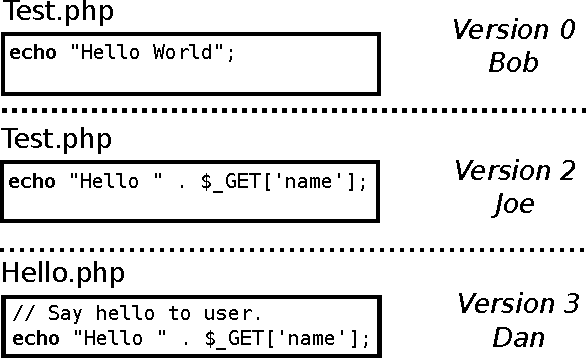
\includegraphics[width=1\linewidth,keepaspectratio]{data/figures/history.pdf}
	\caption{Example of a project history. The project is composed of only one file \texttt{Test.php} which is renamed to \texttt{Hello.php} in the last version.}
	\label{fig:history}
\end{figure}

If renaming is not taken into account, the last version of the project of \figref{history} contains only one file, that has only one version. Therefore its code churn is $2$ (it has 2 lines of codes), and the number of developers and modification is $1$. However, if renaming is taken into account, the last version of the project contains one file that has $3$ versions. In this case the code churn is $4$ ($1$ for version 1, $2$ for version 2 and $1$ for version $3$). The number of developers and modifications are $3$. Therefore this small example shows the importance of taking renaming into account.

\section{Methodology}
\subsection{Where do we look ?}
We want to compare the proportion and the quantity of renames detected by git in this 3 pieces of the software:\\
The Maintenance part, the Development part and the Initialisation part. Plus we want to divide the Development part by major releases.\\
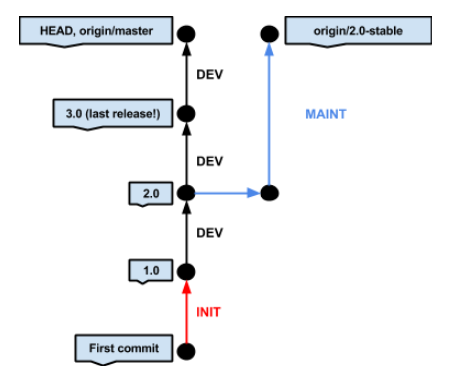
\includegraphics[scale=0.5]{illustrations/draw1}\\
Three types:\\
\textbf{MAINT:} Caintenance branch, a branch which has its head out of master branch. Only commits which are reachable from the branch and not from master.\\
\textbf{INIT:} Commits from the first one (included) to the first major release tag on branch master.\\
\textbf{DEV:} Commits between this major release tag to the next one on branch master.\\
\textbf{(last release!):} commits from the last major release tag to HEAD.\\
\label{subsec:Where do we look ?}
\subsection{Measures}
We will define here the measure we want to observe on the history of the projects creation.\\\\	
\textbf{Number of files (\#F):} number of files in the whole project at the head of branch , respectively end of release (=beginning to next release)\\
\textbf{Number of active files (\#AF):} number of files active (=created or deleted or copied or modified or renamed) in this branch, resp. release.\\
\textbf{Percentage of active files:\\}
\[ \%AF = \frac{\#AF}{\#F} \] \\
\textbf{Number of modification operations (\#MO):}  number of modifications (=create, delete, copy, rename, modif) on files recorded in the branch, resp. release.\\
\textbf{Number of rename operations (\#RO):} number of renames recorded on the branch, resp. release\\
\textbf{Percentage of rename operations :}\\
\[ \%RO = \frac{\#RO}{\#MO}  \] \\
\textbf{Percentage of files renamed:}\\
\[ \%F_{R} = \frac{\#AF_{R}}{\#F} \] \\
this give us the proportion of all files in the project renamed in this branch, resp. release and shows its impact on the whole project.\\
\textbf{Percentage of active files renamed:}
\[ \%AF_{R} = \frac{\#AF_{R}}{\#AF} \]\\
this give us the proportion of active files in the branch, resp. release, renamed in the branch, resp. release. So \[ \%AFR \geq \%FR \] \\
\label{subsec:Measures}

\subsection{Process}

We will describe here the process to follow to obtain this numbers considering any git repository which follows our model. A Ruby script implementation of the following process is given in annexe.\\
First of all we need to list major releases tags in a chronological ascending order. This part can not be automated because of the different tag conventions between projetcs like:
\begin{itemize}
\item PHPunit: 3.5.0, 3.6.0 etc. 
\item Pyramid: 1.0, 1.1 etc.
\item Jenkins: jenkins-1\_400,  jenkins-1\_410 etc.
\item Rails: v2.0.0, v2.1.0 etc. 
\end{itemize}
\medskip
Begin the process:\\
We list the project remotes branches. Browsing the branches, all of them we be considered as maintenance branch except origin/master, the initial and developement branch. Most of the time, specific maintenance branches are followed by “stable”. But if the branch is listed here, it means it has it’s head out of master branch and so it is a maintenance branch since its last merge with master.\\\\
The work is divided in two major step:
\begin{itemize}
\item The maintenance branches
\item origin/master
\end{itemize}
\medskip
If the branch is origin/master, the work will be divided again in:
\begin{itemize}
\item first commit(included) to first release tag
\item fisrt tag to last tag (one release after another)
\item last tag to HEAD
\end{itemize}
\medskip
So in any of the four conditions, we will generate the git log between revision range.
The major part of the work will be on this commits log. We choosed to work on a general log more than mining the history of every files one after the other for performance reasons. Especially on big projects (rails, jenkins). Moreover this technique only works for the files alive at the HEAD of the project and not from one previous revision. So we analyse all the log in one block, with the good command and options it contains enough informations. Log lines stored in simple structures like arrays, we can easily count modifications or renames detected.\\
We will also need to get all the alive files at the end of the log, at the second revision range (branch head or the end of one release).\\\\
Then the principal algorithm will browse the log :\\
Browsing the log in a chronological order will allow us to follow the renames or modifications and rebuilt the history of files.
The typical rename in the log looks like ''rename bob/\{henry $\Rightarrow$ josef\}/george.py (86\%)''
As exemple, if ''bob/henry/george.py'' is already recorded, we need to follow ''bob/josef/george.py'' instead in the renames and modifications record.
There is some other cases to consider, for exemple ''\{henry $\Rightarrow$ \}'' or without ''\{'' or the ''copy'' etc.\\
Each files recorded are unique and only the last name of renamed files is considered.
We finally need exclude all the files deleted before the end of the commits log comparing with the list of alive files at the end of the revision range calculated earlier.\\ 	
\label{subsec:Process}
		
\label{sec:methodology}

\section{Results}
\label{sec:results}

\subsection{First Experiment}

The results of the first experiment are shown in \tabref{jenkins}, \tabref{jquery}, \tabref{phpunit}, \tabref{pyramid} and \tabref{rails}. These tables show several interesting particularities. Firstly, the amount of renaming vary a lot between projects and release. For instance Jenkins has at most $10\%$ of its files renamed in the worst period while PHPUnit has $98.51\%$. In general, there is a large amount of periods with $0\%$ of renamed files.

Regarding the location, the init period seems to be the worst one. It generally has the greater percentage of renamed files (except in PHPUnit). The dev periods are more prone to renaming than the maint periods, as all five projects have close to $0\%$ of renamed files in maint periods. Finally dev periods can contain a lot of renaming. The results seems to indicate that the major releases are the worse.

\begin{table}
\centering
\small
\csvreader[tabular=lcccccc, table head=\toprule Name & Kind & $\#F$ & $\#AF$ & $\%AF$ & $\%F_r$ & $\%AF_r$\\\midrule, late after line=\\, late after last line=\\\bottomrule, after table=]{data/tables/jenkins.csv}%
{1=\name,2=\kind,3=\nf,4=\naf,5=\paf,6=\pfr,7=\pafr}%
{\emph{\name} & \kind & \nf & \naf & \paf & \pfr & \pafr}
\caption{Amount and location of renaming in Jenkins}
\label{tab:jenkins}
\end{table}

\begin{table}
\centering
\small
\csvreader[tabular=lcccccc, table head=\toprule Name & Kind & $\#F$ & $\#AF$ & $\%AF$ & $\%F_r$ & $\%AF_r$\\\midrule, late after line=\\, late after last line=\\\bottomrule]{data/tables/jquery.csv}%
{1=\name,2=\kind,3=\nf,4=\naf,5=\paf,6=\pfr,7=\pafr}%
{\emph{\name} & \kind & \nf & \naf & \paf & \pfr & \pafr}
\caption{Amount and location of renaming in JQuery}
\label{tab:jquery}
\end{table}

\begin{table}
\centering
\small
\csvreader[tabular=lcccccc, table head=\toprule Name & Kind & $\#F$ & $\#AF$ & $\%AF$ & $\%F_r$ & $\%AF_r$\\\midrule, late after line=\\, late after last line=\\\bottomrule]{data/tables/phpunit.csv}%
{1=\name,2=\kind,3=\nf,4=\naf,5=\paf,6=\pfr,7=\pafr}%
{\emph{\name} & \kind & \nf & \naf & \paf & \pfr & \pafr}
\caption{Amount and location of renaming in PHPUnit}
\label{tab:phpunit}
\end{table}

\begin{table}
\centering
\small
\csvreader[tabular=lcccccc, table head=\toprule Name & Kind & $\#F$ & $\#AF$ & $\%AF$ & $\%F_r$ & $\%AF_r$\\\midrule, late after line=\\, late after last line=\\\bottomrule]{data/tables/pyramid.csv}%
{1=\name,2=\kind,3=\nf,4=\naf,5=\paf,6=\pfr,7=\pafr}%
{\emph{\name} & \kind & \nf & \naf & \paf & \pfr & \pafr}
\caption{Amount and location of renaming in Pyramid}
\label{tab:pyramid}
\end{table}

\begin{table}
\centering
\small
\csvreader[tabular=lcccccc, table head=\toprule Name & Kind & $\#F$ & $\#AF$ & $\%AF$ & $\%F_r$ & $\%AF_r$\\\midrule, late after line=\\, late after last line=\\\bottomrule]{data/tables/rails.csv}%
{1=\name,2=\kind,3=\nf,4=\naf,5=\paf,6=\pfr,7=\pafr}%
{\emph{\name} & \kind & \nf & \naf & \paf & \pfr & \pafr}
\caption{Amount and location of renaming in Rails}
\label{tab:rails}
\end{table}

\subsection{Second Experiment}

\begin{table*}
\centering
\small
\begin{tabular}{lcccc}
\toprule
Period & Code churn & Nb of developers & Nb of modifications\\
\midrule
PHPUnit 3.7.0-4.0.0 & 0.60 & 0.4 & 0.60\\
\bottomrule
\end{tabular}
\caption{Spearman correlation coefficients between values of change metrics with and without renaming.}
\label{tab:spearman}
\end{table*}
\section{Analysis of Past Studies}
\label{sec:study}

In this section, we proceed to an analysis of the past studies that used change metrics to predict defects. We evaluate if the values of changes metrics could be biased by analyzing how they collected their data. Finally, we give some guidelines to help researchers and practitioners to avoid the impact that artifact renaming has on change metrics.

\subsection{Analysis of Past Studies}

Firstly, it is important to remark that as we have shown in \secref{results}, periods containing a high amount of renaming are rare. Therefore, most of the past studies should be not affected by this phenomenon. Additionally, even in the case of using periods having a significant amount of renaming, the results of such studies could also be improved, because change metrics would probably have been underestimated. Nevertheless, several past studies can be impacted by renaming, as we will point out in the remainder of this section. Quantifying such effect on these past studies is out of the scope of this paper, but we provide guidelines for future studies in \secref{guidelines}.

In this analysis of past studies, we include only the 26 studies referenced in~\cite{radjenovic_software_2013} that use the CC, NoD or NoC metrics. However several other studies referenced in~\cite{radjenovic_software_2013} use slightly different change metrics and could also be impacted on renaming.

$15$ past studies use industrial software projects~\cite{arisholm_systematic_2010,graves_predicting_2000,khoshgoftaar_using_2000,layman_iterative_2008,munson_code_1998,nagappan_use_2005,nagappan_influence_2008,nagappan_using_2007,nagappan_using_2006,nagappan_change_2010,nikora_building_2006,ostrand_programmer-based_2010,weyuker_too_2008,weyuker_using_2007,yuan_application_2000}. All these studies did not list artifact renaming anywhere in the data collection or threats to validity sections. Unfortunately, the lack of information about VCSs and software projects used in these studies forbid us to evaluate if artifact renaming is a possible bias for their result. However, the article of Kim et al.~\cite{kim_field_2012} points out the fact that industrial developers can also perform refactoring (including renaming) without using the dedicated tool. Therefore these studies might be impacted depending on the tools and habits of developers involved in the industrial projects.

$11$ studies use open-source software projects\cite{dambros_relationship_2009,bacchelli_are_2010,caglayan_merits_2009,dambros_evaluating_2012,dambros_evaluating_2012,dambros_extensive_2010,illes-seifert_exploring_2010,li_finding_2005,matsumoto_analysis_2010,moser_analysis_2008,moser_comparative_2008,schroter_if_2006}. The VCSs used by the projects included in these studies are either CVS or Subversion. CVS do not handle renaming, and Subversion handles renaming manually which is dangerous as explained in~\cite{lavoie_inferring_2012,steidl_incremental_2014}. However, only $2$ of these studies~\cite{moser_analysis_2008,moser_comparative_2008} listed artifact renaming in their data collection or threat to validity sections. To mitigate the risk of artifact renaming, these 2 studies deleted from their corpus files that have been added or removed during the analyzed periods. This is an effective way of avoiding computing skewed change metric values. However, it can remove unnecessarily a significant amount of files from the corpus, which in turn might bias the study. In conclusion, all these studies might also be impacted by artifact renaming.

\subsection{Guidelines}
\label{sec:guidelines}

According to the results of our two experiments, we deduce several simple guidelines to compute change metrics. Firstly, we recommend to avoid computing such metrics during initial periods of projects at all costs. Indeed, these periods usually contain a significant amount of renaming. As we have seen, both major and minor periods can contain a significant amount of renaming, although major release seems more prone to renaming. In any case, we recommend to systematically use a renaming detection algorithm, to avoid picking up the wrong period. Git provides a dedicated algorithm that seems to have a good precision, but an unknown recall. Therefore using projects managed by Git seems the easier way to lower the threat of renaming. More advanced renaming detection algorithms are also described in the literature:~\cite{antoniol_automatic_2004,lavoie_inferring_2012,steidl_incremental_2014}. They have been empirically validated so they might perform better than Git's algorithm, and are the only choices if the chosen corpus contains project that are not managed by Git. Finally, for change metrics computed at finer level of granularity than files, we recommend the use of origin analysis algorithms such as~\cite{wu_aura:_2010}. These algorithms usually work at the granularity of the functions. Finally, as artifact renaming can be a significant threat, we recommend to systematically indicate how it was dealt with in future studies.

\section{Conclusion}
\label{sec:conclusion}

Dans cet article, nous avons évalué l'impact du renommage d'entités sur les valeurs des métriques de procédés logicielles. Nous avons effectué une étude empirique sur cinq projets open-source connus et matures. Nous avons observé que les périodes initiales des projets sont plus enclines à contenir du renommage que les autres périodes. Plus important, nous avons constaté que d'autres périodes peuvent contenir une quantité importante de renommage, en particulier celles correspondantes à la mise au point de releases majeures. Enfin, nous avons observé que le renommage pouvait biaiser considérablement les valeurs des métriques de procédés. Par conséquent, les chercheurs et développeurs devraient être prudent lors du calcul des métriques de procédés. Nous recommandons d'éviter le calcul des métriques de procédés lors des périodes initiales. Pour finir, nous recommandons fortement d'utiliser un algorithme de détection de renommage lors du calcul des métriques de procédés sur d'autres périodes tels qu'il pourrait en biaiser fortement le résultat.\\

A l'avenir, nous prévoyons d'évaluer la précision des algorithmes existants de détection de renommage. Nous prévoyons également d'évaluer l'impact de la fusion de code (code merging) sur les métriques de procédés.


\bibliographystyle{IEEEtran}
\bibliography{renaming}

\end{document}
